\documentclass[1p]{elsarticle_modified}
%\bibliographystyle{elsarticle-num}

%\usepackage[colorlinks]{hyperref}
%\usepackage{abbrmath_seonhwa} %\Abb, \Ascr, \Acal ,\Abf, \Afrak
\usepackage{amsfonts}
\usepackage{amssymb}
\usepackage{amsmath}
\usepackage{amsthm}
\usepackage{scalefnt}
\usepackage{amsbsy}
\usepackage{kotex}
\usepackage{caption}
\usepackage{subfig}
\usepackage{color}
\usepackage{graphicx}
\usepackage{xcolor} %% white, black, red, green, blue, cyan, magenta, yellow
\usepackage{float}
\usepackage{setspace}
\usepackage{hyperref}

\usepackage{tikz}
\usetikzlibrary{arrows}

\usepackage{multirow}
\usepackage{array} % fixed length table
\usepackage{hhline}

%%%%%%%%%%%%%%%%%%%%%
\makeatletter
\renewcommand*\env@matrix[1][\arraystretch]{%
	\edef\arraystretch{#1}%
	\hskip -\arraycolsep
	\let\@ifnextchar\new@ifnextchar
	\array{*\c@MaxMatrixCols c}}
\makeatother %https://tex.stackexchange.com/questions/14071/how-can-i-increase-the-line-spacing-in-a-matrix
%%%%%%%%%%%%%%%

\usepackage[normalem]{ulem}

\newcommand{\msout}[1]{\ifmmode\text{\sout{\ensuremath{#1}}}\else\sout{#1}\fi}
%SOURCE: \msout is \stkout macro in https://tex.stackexchange.com/questions/20609/strikeout-in-math-mode

\newcommand{\cancel}[1]{
	\ifmmode
	{\color{red}\msout{#1}}
	\else
	{\color{red}\sout{#1}}
	\fi
}

\newcommand{\add}[1]{
	{\color{blue}\uwave{#1}}
}

\newcommand{\replace}[2]{
	\ifmmode
	{\color{red}\msout{#1}}{\color{blue}\uwave{#2}}
	\else
	{\color{red}\sout{#1}}{\color{blue}\uwave{#2}}
	\fi
}

\newcommand{\Sol}{\mathcal{S}} %segment
\newcommand{\D}{D} %diagram
\newcommand{\A}{\mathcal{A}} %arc


%%%%%%%%%%%%%%%%%%%%%%%%%%%%%5 test

\def\sl{\operatorname{\textup{SL}}(2,\Cbb)}
\def\psl{\operatorname{\textup{PSL}}(2,\Cbb)}
\def\quan{\mkern 1mu \triangleright \mkern 1mu}

\theoremstyle{definition}
\newtheorem{thm}{Theorem}[section]
\newtheorem{prop}[thm]{Proposition}
\newtheorem{lem}[thm]{Lemma}
\newtheorem{ques}[thm]{Question}
\newtheorem{cor}[thm]{Corollary}
\newtheorem{defn}[thm]{Definition}
\newtheorem{exam}[thm]{Example}
\newtheorem{rmk}[thm]{Remark}
\newtheorem{alg}[thm]{Algorithm}

\newcommand{\I}{\sqrt{-1}}
\begin{document}

%\begin{frontmatter}
%
%\title{Boundary parabolic representations of knots up to 8 crossings}
%
%%% Group authors per affiliation:
%\author{Yunhi Cho} 
%\address{Department of Mathematics, University of Seoul, Seoul, Korea}
%\ead{yhcho@uos.ac.kr}
%
%
%\author{Seonhwa Kim} %\fnref{s_kim}}
%\address{Center for Geometry and Physics, Institute for Basic Science, Pohang, 37673, Korea}
%\ead{ryeona17@ibs.re.kr}
%
%\author{Hyuk Kim}
%\address{Department of Mathematical Sciences, Seoul National University, Seoul 08826, Korea}
%\ead{hyukkim@snu.ac.kr}
%
%\author{Seokbeom Yoon}
%\address{Department of Mathematical Sciences, Seoul National University, Seoul, 08826,  Korea}
%\ead{sbyoon15@snu.ac.kr}
%
%\begin{abstract}
%We find all boundary parabolic representation of knots up to 8 crossings.
%
%\end{abstract}
%\begin{keyword}
%    \MSC[2010] 57M25 
%\end{keyword}
%
%\end{frontmatter}

%\linenumbers
%\tableofcontents
%
\newcommand\colored[1]{\textcolor{white}{\rule[-0.35ex]{0.8em}{1.4ex}}\kern-0.8em\color{red} #1}%
%\newcommand\colored[1]{\textcolor{white}{ #1}\kern-2.17ex	\textcolor{white}{ #1}\kern-1.81ex	\textcolor{white}{ #1}\kern-2.15ex\color{red}#1	}

{\Large $\underline{12n_{0483}~(K12n_{0483})}$}

\setlength{\tabcolsep}{10pt}
\renewcommand{\arraystretch}{1.6}
\vspace{1cm}\begin{tabular}{m{100pt}>{\centering\arraybackslash}m{274pt}}
\multirow{5}{120pt}{
	\centering
	\includegraphics[width=112pt]{../../../GIT/diagram.site/Diagrams/png/2572_12n_0483.png}\\
\ \ \ A knot diagram\footnotemark}&
\allowdisplaybreaks
\textbf{Linearized knot diagam} \\
\cline{2-2}
 &
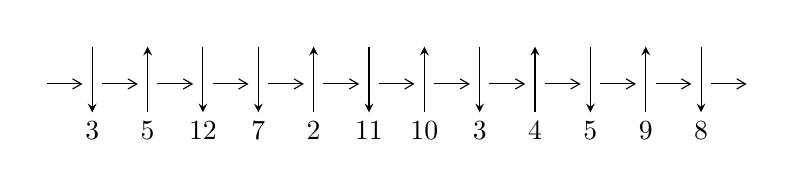
\begin{tikzpicture}[x=20pt, y=17pt]
	% nodes
	\node (C0) at (0, 0) {};
	\node (C1) at (1, 0) {};
	\node (C1U) at (1, +1) {};
	\node (C1D) at (1, -1) {3};

	\node (C2) at (2, 0) {};
	\node (C2U) at (2, +1) {};
	\node (C2D) at (2, -1) {5};

	\node (C3) at (3, 0) {};
	\node (C3U) at (3, +1) {};
	\node (C3D) at (3, -1) {12};

	\node (C4) at (4, 0) {};
	\node (C4U) at (4, +1) {};
	\node (C4D) at (4, -1) {7};

	\node (C5) at (5, 0) {};
	\node (C5U) at (5, +1) {};
	\node (C5D) at (5, -1) {2};

	\node (C6) at (6, 0) {};
	\node (C6U) at (6, +1) {};
	\node (C6D) at (6, -1) {11};

	\node (C7) at (7, 0) {};
	\node (C7U) at (7, +1) {};
	\node (C7D) at (7, -1) {10};

	\node (C8) at (8, 0) {};
	\node (C8U) at (8, +1) {};
	\node (C8D) at (8, -1) {3};

	\node (C9) at (9, 0) {};
	\node (C9U) at (9, +1) {};
	\node (C9D) at (9, -1) {4};

	\node (C10) at (10, 0) {};
	\node (C10U) at (10, +1) {};
	\node (C10D) at (10, -1) {5};

	\node (C11) at (11, 0) {};
	\node (C11U) at (11, +1) {};
	\node (C11D) at (11, -1) {9};

	\node (C12) at (12, 0) {};
	\node (C12U) at (12, +1) {};
	\node (C12D) at (12, -1) {8};
	\node (C13) at (13, 0) {};

	% arrows
	\draw[->,>={angle 60}]
	(C0) edge (C1) (C1) edge (C2) (C2) edge (C3) (C3) edge (C4) (C4) edge (C5) (C5) edge (C6) (C6) edge (C7) (C7) edge (C8) (C8) edge (C9) (C9) edge (C10) (C10) edge (C11) (C11) edge (C12) (C12) edge (C13) ;	\draw[->,>=stealth]
	(C1U) edge (C1D) (C2D) edge (C2U) (C3U) edge (C3D) (C4U) edge (C4D) (C5D) edge (C5U) (C6U) edge (C6D) (C7D) edge (C7U) (C8U) edge (C8D) (C9D) edge (C9U) (C10U) edge (C10D) (C11D) edge (C11U) (C12U) edge (C12D) ;
	\end{tikzpicture} \\
\hhline{~~} \\& 
\textbf{Solving Sequence} \\ \cline{2-2} 
 &
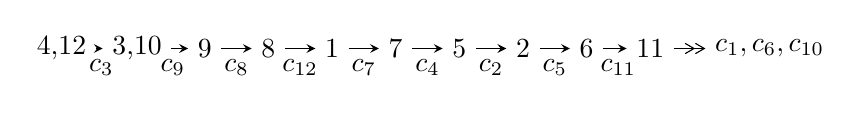
\begin{tikzpicture}[x=23pt, y=7pt]
	% node
	\node (A0) at (-1/8, 0) {4,12};
	\node (A1) at (17/16, 0) {3,10};
	\node (A2) at (17/8, 0) {9};
	\node (A3) at (25/8, 0) {8};
	\node (A4) at (33/8, 0) {1};
	\node (A5) at (41/8, 0) {7};
	\node (A6) at (49/8, 0) {5};
	\node (A7) at (57/8, 0) {2};
	\node (A8) at (65/8, 0) {6};
	\node (A9) at (73/8, 0) {11};
	\node (C1) at (1/2, -1) {$c_{3}$};
	\node (C2) at (13/8, -1) {$c_{9}$};
	\node (C3) at (21/8, -1) {$c_{8}$};
	\node (C4) at (29/8, -1) {$c_{12}$};
	\node (C5) at (37/8, -1) {$c_{7}$};
	\node (C6) at (45/8, -1) {$c_{4}$};
	\node (C7) at (53/8, -1) {$c_{2}$};
	\node (C8) at (61/8, -1) {$c_{5}$};
	\node (C9) at (69/8, -1) {$c_{11}$};
	\node (A10) at (11, 0) {$c_{1},c_{6},c_{10}$};

	% edge
	\draw[->,>=stealth]	
	(A0) edge (A1) (A1) edge (A2) (A2) edge (A3) (A3) edge (A4) (A4) edge (A5) (A5) edge (A6) (A6) edge (A7) (A7) edge (A8) (A8) edge (A9) ;
	\draw[->>,>={angle 60}]	
	(A9) edge (A10);
\end{tikzpicture} \\ 

\end{tabular} \\

\footnotetext{
The image of knot diagram is generated by the software ``\textbf{Draw programme}" developed by Andrew Bartholomew(\url{http://www.layer8.co.uk/maths/draw/index.htm\#Running-draw}), where we modified some parts for our purpose(\url{https://github.com/CATsTAILs/LinksPainter}).
}\phantom \\ \newline 
\centering \textbf{Ideals for irreducible components\footnotemark of $X_{\text{par}}$} 
 
\begin{align*}
I^u_{1}&=\langle 
u^7+u^4+2 u^3+2 u^2+b,\;- u^5- u^2+a-2 u-1,\\
\phantom{I^u_{1}}&\phantom{= \langle  }u^{12}- u^{11}+u^{10}+2 u^9+2 u^8+2 u^7+u^6+5 u^5+6 u^4+3 u^3+2 u^2+u+1\rangle \\
I^u_{2}&=\langle 
u^{17}+7 u^{16}+\cdots+b-1,\;6 u^{17}+47 u^{16}+\cdots+a+12,\;u^{18}+8 u^{17}+\cdots+5 u+1\rangle \\
I^u_{3}&=\langle 
15 u^{13}-39 u^{12}+\cdots+b-29,\;-49 u^{13}+118 u^{12}+\cdots+a+75,\\
\phantom{I^u_{3}}&\phantom{= \langle  }u^{14}-3 u^{13}+4 u^{12}-3 u^{11}+9 u^{10}-21 u^9+22 u^8-7 u^7+7 u^6-31 u^5+48 u^4-41 u^3+22 u^2-7 u+1\rangle \\
I^u_{4}&=\langle 
b,\;a+1,\;u+1\rangle \\
\\
\end{align*}
\raggedright * 4 irreducible components of $\dim_{\mathbb{C}}=0$, with total 45 representations.\\
\footnotetext{All coefficients of polynomials are rational numbers. But the coefficients are sometimes approximated in decimal forms when there is not enough margin.}
\newpage
\renewcommand{\arraystretch}{1}
\centering \section*{I. $I^u_{1}= \langle u^7+u^4+2 u^3+2 u^2+b,\;- u^5- u^2+a-2 u-1,\;u^{12}- u^{11}+\cdots+u+1 \rangle$}
\flushleft \textbf{(i) Arc colorings}\\
\begin{tabular}{m{7pt} m{180pt} m{7pt} m{180pt} }
\flushright $a_{4}=$&$\begin{pmatrix}1\\0\end{pmatrix}$ \\
\flushright $a_{12}=$&$\begin{pmatrix}0\\u\end{pmatrix}$ \\
\flushright $a_{3}=$&$\begin{pmatrix}1\\- u^2\end{pmatrix}$ \\
\flushright $a_{10}=$&$\begin{pmatrix}u^5+u^2+2 u+1\\- u^7- u^4-2 u^3-2 u^2\end{pmatrix}$ \\
\flushright $a_{9}=$&$\begin{pmatrix}u^7+u^5+u^4+2 u^3+3 u^2+2 u+1\\- u^7- u^4-2 u^3-2 u^2\end{pmatrix}$ \\
\flushright $a_{8}=$&$\begin{pmatrix}u^9+u^7+u^6+3 u^5+3 u^4+2 u^3+2 u^2+2 u+1\\- u^{11}- u^8-3 u^7-2 u^6-2 u^3-2 u^2\end{pmatrix}$ \\
\flushright $a_{1}=$&$\begin{pmatrix}- u^{11}- u^9-2 u^8-3 u^7-4 u^6-2 u^5-4 u^4-3 u^3-2 u^2\\- u^{10}- u^9- u^8-3 u^7-4 u^6-7 u^5-5 u^4-4 u^3-3 u^2- u-1\end{pmatrix}$ \\
\flushright $a_{7}=$&$\begin{pmatrix}u^{11}- u^{10}+u^9+u^8+3 u^7+u^6+4 u^4+5 u^3+3 u^2+u\\u\end{pmatrix}$ \\
\flushright $a_{5}=$&$\begin{pmatrix}- u^9+u^8- u^7- u^6- u^5- u^4- u^2- u\\u^2\end{pmatrix}$ \\
\flushright $a_{2}=$&$\begin{pmatrix}- u^9- u^8- u^7-2 u^6-3 u^5-6 u^4-4 u^3-2 u^2- u\\u^{10}+u^9+u^8+u^7+4 u^6+5 u^5+4 u^4+2 u^3+u\end{pmatrix}$ \\
\flushright $a_{6}=$&$\begin{pmatrix}u^{11}+u^{10}+u^9+2 u^8+3 u^7+5 u^6+4 u^5+2 u^4+u^3+u^2\\u^{10}+u^9+u^8+3 u^7+4 u^6+7 u^5+5 u^4+4 u^3+3 u^2+u+1\end{pmatrix}$ \\
\flushright $a_{11}=$&$\begin{pmatrix}u^{10}+u^7+2 u^6+3 u^5- u^4- u^3+u^2+2 u+1\\- u^{11}- u^8-3 u^7-2 u^6-2 u^3-2 u^2\end{pmatrix}$\\&\end{tabular}
\flushleft \textbf{(ii) Obstruction class $= -1$}\\~\\
\flushleft \textbf{(iii) Cusp Shapes $= -4 u^{11}+6 u^{10}-6 u^9-6 u^8-6 u^7-2 u^6-2 u^5-20 u^4-14 u^3-2 u^2-2 u-2$}\\~\\
\newpage\renewcommand{\arraystretch}{1}
\flushleft \textbf{(iv) u-Polynomials at the component}\newline \\
\begin{tabular}{m{50pt}|m{274pt}}
Crossings & \hspace{64pt}u-Polynomials at each crossing \\
\hline $$\begin{aligned}c_{1}\end{aligned}$$&$\begin{aligned}
&u^{12}+36 u^{11}+\cdots+10212 u+784
\end{aligned}$\\
\hline $$\begin{aligned}c_{2},c_{5}\end{aligned}$$&$\begin{aligned}
&u^{12}+4 u^{11}+\cdots+34 u+28
\end{aligned}$\\
\hline $$\begin{aligned}c_{3},c_{4}\end{aligned}$$&$\begin{aligned}
&u^{12}- u^{11}+u^{10}+2 u^9+2 u^8+2 u^7+u^6+5 u^5+6 u^4+3 u^3+2 u^2+u+1
\end{aligned}$\\
\hline $$\begin{aligned}c_{6},c_{12}\end{aligned}$$&$\begin{aligned}
&u^{12}- u^{11}+\cdots-112 u+16
\end{aligned}$\\
\hline $$\begin{aligned}c_{7},c_{11}\end{aligned}$$&$\begin{aligned}
&u^{12}+u^{11}+\cdots+3 u+1
\end{aligned}$\\
\hline $$\begin{aligned}c_{8},c_{10}\end{aligned}$$&$\begin{aligned}
&u^{12}- u^{11}+\cdots- u+1
\end{aligned}$\\
\hline $$\begin{aligned}c_{9}\end{aligned}$$&$\begin{aligned}
&u^{12}+8 u^{11}+\cdots+32 u+8
\end{aligned}$\\
\hline
\end{tabular}\\~\\
\newpage\renewcommand{\arraystretch}{1}
\flushleft \textbf{(v) Riley Polynomials at the component}\newline \\
\begin{tabular}{m{50pt}|m{274pt}}
Crossings & \hspace{64pt}Riley Polynomials at each crossing \\
\hline $$\begin{aligned}c_{1}\end{aligned}$$&$\begin{aligned}
&y^{12}-104 y^{11}+\cdots-27451376 y+614656
\end{aligned}$\\
\hline $$\begin{aligned}c_{2},c_{5}\end{aligned}$$&$\begin{aligned}
&y^{12}+36 y^{11}+\cdots+10212 y+784
\end{aligned}$\\
\hline $$\begin{aligned}c_{3},c_{4}\end{aligned}$$&$\begin{aligned}
&y^{12}+y^{11}+\cdots+3 y+1
\end{aligned}$\\
\hline $$\begin{aligned}c_{6},c_{12}\end{aligned}$$&$\begin{aligned}
&y^{12}-35 y^{11}+\cdots+1280 y+256
\end{aligned}$\\
\hline $$\begin{aligned}c_{7},c_{11}\end{aligned}$$&$\begin{aligned}
&y^{12}+11 y^{11}+\cdots+175 y+1
\end{aligned}$\\
\hline $$\begin{aligned}c_{8},c_{10}\end{aligned}$$&$\begin{aligned}
&y^{12}-25 y^{11}+\cdots+21 y+1
\end{aligned}$\\
\hline $$\begin{aligned}c_{9}\end{aligned}$$&$\begin{aligned}
&y^{12}-6 y^{11}+\cdots+160 y+64
\end{aligned}$\\
\hline
\end{tabular}\\~\\
\newpage\flushleft \textbf{(vi) Complex Volumes and Cusp Shapes}
$$\begin{array}{c|c|c}  
\text{Solutions to }I^u_{1}& \I (\text{vol} + \sqrt{-1}CS) & \text{Cusp shape}\\
 \hline 
\begin{aligned}
u &= -0.943494 + 0.203851 I \\
a &= -0.445140 + 0.755661 I \\
b &= -0.761544 - 0.427838 I\end{aligned}
 & -1.86414 + 1.86169 I & -7.41273 - 3.81862 I \\ \hline\begin{aligned}
u &= -0.943494 - 0.203851 I \\
a &= -0.445140 - 0.755661 I \\
b &= -0.761544 + 0.427838 I\end{aligned}
 & -1.86414 - 1.86169 I & -7.41273 + 3.81862 I \\ \hline\begin{aligned}
u &= -0.428222 + 0.989663 I \\
a &= -1.95175 + 0.47004 I \\
b &= -1.156050 - 0.432518 I\end{aligned}
 & \phantom{-}2.66700 + 5.59294 I & \phantom{-}4.27657 - 7.89716 I \\ \hline\begin{aligned}
u &= -0.428222 - 0.989663 I \\
a &= -1.95175 - 0.47004 I \\
b &= -1.156050 + 0.432518 I\end{aligned}
 & \phantom{-}2.66700 - 5.59294 I & \phantom{-}4.27657 + 7.89716 I \\ \hline\begin{aligned}
u &= -0.433065 + 0.576514 I \\
a &= \phantom{-}0.004562 + 0.459402 I \\
b &= -0.083913 + 0.568146 I\end{aligned}
 & -0.34049 + 1.65634 I & -1.46994 - 4.66889 I \\ \hline\begin{aligned}
u &= -0.433065 - 0.576514 I \\
a &= \phantom{-}0.004562 - 0.459402 I \\
b &= -0.083913 - 0.568146 I\end{aligned}
 & -0.34049 - 1.65634 I & -1.46994 + 4.66889 I \\ \hline\begin{aligned}
u &= \phantom{-}0.308633 + 0.557970 I \\
a &= \phantom{-}1.46204 + 1.37428 I \\
b &= \phantom{-}1.005310 - 0.551014 I\end{aligned}
 & \phantom{-}1.99940 - 1.87880 I & \phantom{-}2.68729 + 1.13887 I \\ \hline\begin{aligned}
u &= \phantom{-}0.308633 - 0.557970 I \\
a &= \phantom{-}1.46204 - 1.37428 I \\
b &= \phantom{-}1.005310 + 0.551014 I\end{aligned}
 & \phantom{-}1.99940 + 1.87880 I & \phantom{-}2.68729 - 1.13887 I \\ \hline\begin{aligned}
u &= \phantom{-}0.96431 + 1.04939 I \\
a &= -0.436521 - 0.813671 I \\
b &= -1.55023 - 1.27982 I\end{aligned}
 & -18.7687 - 2.1933 I & -2.97846 + 2.17261 I \\ \hline\begin{aligned}
u &= \phantom{-}0.96431 - 1.04939 I \\
a &= -0.436521 + 0.813671 I \\
b &= -1.55023 + 1.27982 I\end{aligned}
 & -18.7687 + 2.1933 I & -2.97846 - 2.17261 I\\
 \hline 
 \end{array}$$\newpage$$\begin{array}{c|c|c}  
\text{Solutions to }I^u_{1}& \I (\text{vol} + \sqrt{-1}CS) & \text{Cusp shape}\\
 \hline 
\begin{aligned}
u &= \phantom{-}1.03184 + 1.04165 I \\
a &= -1.63319 - 0.67021 I \\
b &= -1.45358 + 1.34749 I\end{aligned}
 & -19.0592 - 12.8315 I & -3.10274 + 5.68817 I \\ \hline\begin{aligned}
u &= \phantom{-}1.03184 - 1.04165 I \\
a &= -1.63319 + 0.67021 I \\
b &= -1.45358 - 1.34749 I\end{aligned}
 & -19.0592 + 12.8315 I & -3.10274 - 5.68817 I\\
 \hline 
 \end{array}$$\newpage\newpage\renewcommand{\arraystretch}{1}
\centering \section*{II. $I^u_{2}= \langle u^{17}+7 u^{16}+\cdots+b-1,\;6 u^{17}+47 u^{16}+\cdots+a+12,\;u^{18}+8 u^{17}+\cdots+5 u+1 \rangle$}
\flushleft \textbf{(i) Arc colorings}\\
\begin{tabular}{m{7pt} m{180pt} m{7pt} m{180pt} }
\flushright $a_{4}=$&$\begin{pmatrix}1\\0\end{pmatrix}$ \\
\flushright $a_{12}=$&$\begin{pmatrix}0\\u\end{pmatrix}$ \\
\flushright $a_{3}=$&$\begin{pmatrix}1\\- u^2\end{pmatrix}$ \\
\flushright $a_{10}=$&$\begin{pmatrix}-6 u^{17}-47 u^{16}+\cdots-50 u-12\\- u^{17}-7 u^{16}+\cdots- u+1\end{pmatrix}$ \\
\flushright $a_{9}=$&$\begin{pmatrix}-5 u^{17}-40 u^{16}+\cdots-49 u-13\\- u^{17}-7 u^{16}+\cdots- u+1\end{pmatrix}$ \\
\flushright $a_{8}=$&$\begin{pmatrix}-5 u^{17}-39 u^{16}+\cdots-45 u-12\\u^{16}+7 u^{15}+\cdots+4 u+2\end{pmatrix}$ \\
\flushright $a_{1}=$&$\begin{pmatrix}13 u^{17}+99 u^{16}+\cdots+84 u+19\\-2 u^{17}-16 u^{16}+\cdots-18 u-6\end{pmatrix}$ \\
\flushright $a_{7}=$&$\begin{pmatrix}3 u^{17}+19 u^{16}+\cdots-11 u-8\\-5 u^{17}-38 u^{16}+\cdots-29 u-6\end{pmatrix}$ \\
\flushright $a_{5}=$&$\begin{pmatrix}21 u^{17}+156 u^{16}+\cdots+111 u+22\\-6 u^{17}-48 u^{16}+\cdots-45 u-12\end{pmatrix}$ \\
\flushright $a_{2}=$&$\begin{pmatrix}14 u^{17}+107 u^{16}+\cdots+90 u+20\\- u^{17}-9 u^{16}+\cdots-17 u-6\end{pmatrix}$ \\
\flushright $a_{6}=$&$\begin{pmatrix}33 u^{17}+249 u^{16}+\cdots+195 u+43\\-5 u^{17}-42 u^{16}+\cdots-54 u-16\end{pmatrix}$ \\
\flushright $a_{11}=$&$\begin{pmatrix}18 u^{17}+137 u^{16}+\cdots+109 u+23\\-3 u^{17}-26 u^{16}+\cdots-34 u-10\end{pmatrix}$\\&\end{tabular}
\flushleft \textbf{(ii) Obstruction class $= 1$}\\~\\
\flushleft \textbf{(iii) Cusp Shapes $= -36 u^{17}-268 u^{16}-1035 u^{15}-2527 u^{14}-4242 u^{13}-4893 u^{12}-3632 u^{11}-1032 u^{10}+1235 u^9+2183 u^8+1783 u^7+724 u^6-361 u^5-832 u^4-748 u^3-435 u^2-188 u-40$}\\~\\
\newpage\renewcommand{\arraystretch}{1}
\flushleft \textbf{(iv) u-Polynomials at the component}\newline \\
\begin{tabular}{m{50pt}|m{274pt}}
Crossings & \hspace{64pt}u-Polynomials at each crossing \\
\hline $$\begin{aligned}c_{1}\end{aligned}$$&$\begin{aligned}
&(u^9-5 u^8+11 u^7-5 u^6-6 u^5+6 u^4+3 u^3-4 u^2+1)^2
\end{aligned}$\\
\hline $$\begin{aligned}c_{2}\end{aligned}$$&$\begin{aligned}
&(u^9- u^8+3 u^7- u^6+2 u^5-2 u^4- u^3+1)^2
\end{aligned}$\\
\hline $$\begin{aligned}c_{3}\end{aligned}$$&$\begin{aligned}
&u^{18}+8 u^{17}+\cdots+5 u+1
\end{aligned}$\\
\hline $$\begin{aligned}c_{4}\end{aligned}$$&$\begin{aligned}
&u^{18}-8 u^{17}+\cdots-5 u+1
\end{aligned}$\\
\hline $$\begin{aligned}c_{5}\end{aligned}$$&$\begin{aligned}
&(u^9+u^8+3 u^7+u^6+2 u^5+2 u^4- u^3-1)^2
\end{aligned}$\\
\hline $$\begin{aligned}c_{6}\end{aligned}$$&$\begin{aligned}
&u^{18}+4 u^{17}+\cdots-64 u+16
\end{aligned}$\\
\hline $$\begin{aligned}c_{7}\end{aligned}$$&$\begin{aligned}
&u^{18}+5 u^{17}+\cdots+6 u+1
\end{aligned}$\\
\hline $$\begin{aligned}c_{8}\end{aligned}$$&$\begin{aligned}
&u^{18}+2 u^{17}+\cdots- u+1
\end{aligned}$\\
\hline $$\begin{aligned}c_{9}\end{aligned}$$&$\begin{aligned}
&u^{18}-6 u^{16}+18 u^{14}-32 u^{12}+36 u^{10}-21 u^8- u^6+13 u^4-9 u^2+2
\end{aligned}$\\
\hline $$\begin{aligned}c_{10}\end{aligned}$$&$\begin{aligned}
&u^{18}-2 u^{17}+\cdots+u+1
\end{aligned}$\\
\hline $$\begin{aligned}c_{11}\end{aligned}$$&$\begin{aligned}
&u^{18}-5 u^{17}+\cdots-6 u+1
\end{aligned}$\\
\hline $$\begin{aligned}c_{12}\end{aligned}$$&$\begin{aligned}
&u^{18}-4 u^{17}+\cdots+64 u+16
\end{aligned}$\\
\hline
\end{tabular}\\~\\
\newpage\renewcommand{\arraystretch}{1}
\flushleft \textbf{(v) Riley Polynomials at the component}\newline \\
\begin{tabular}{m{50pt}|m{274pt}}
Crossings & \hspace{64pt}Riley Polynomials at each crossing \\
\hline $$\begin{aligned}c_{1}\end{aligned}$$&$\begin{aligned}
&(y^9-3 y^8+59 y^7-91 y^6+122 y^5-102 y^4+67 y^3-28 y^2+8 y-1)^2
\end{aligned}$\\
\hline $$\begin{aligned}c_{2},c_{5}\end{aligned}$$&$\begin{aligned}
&(y^9+5 y^8+11 y^7+5 y^6-6 y^5-6 y^4+3 y^3+4 y^2-1)^2
\end{aligned}$\\
\hline $$\begin{aligned}c_{3},c_{4}\end{aligned}$$&$\begin{aligned}
&y^{18}+2 y^{17}+\cdots+3 y+1
\end{aligned}$\\
\hline $$\begin{aligned}c_{6},c_{12}\end{aligned}$$&$\begin{aligned}
&y^{18}-22 y^{17}+\cdots-512 y+256
\end{aligned}$\\
\hline $$\begin{aligned}c_{7},c_{11}\end{aligned}$$&$\begin{aligned}
&y^{18}-9 y^{17}+\cdots-4 y+1
\end{aligned}$\\
\hline $$\begin{aligned}c_{8},c_{10}\end{aligned}$$&$\begin{aligned}
&y^{18}-8 y^{17}+\cdots- y+1
\end{aligned}$\\
\hline $$\begin{aligned}c_{9}\end{aligned}$$&$\begin{aligned}
&(y^9-6 y^8+18 y^7-32 y^6+36 y^5-21 y^4- y^3+13 y^2-9 y+2)^2
\end{aligned}$\\
\hline
\end{tabular}\\~\\
\newpage\flushleft \textbf{(vi) Complex Volumes and Cusp Shapes}
$$\begin{array}{c|c|c}  
\text{Solutions to }I^u_{2}& \I (\text{vol} + \sqrt{-1}CS) & \text{Cusp shape}\\
 \hline 
\begin{aligned}
u &= -0.777312 + 0.486718 I \\
a &= -0.117694 - 0.428312 I \\
b &= \phantom{-0.000000 -}0.824936 I\end{aligned}
 & -2.92265\phantom{ +0.000000I} & -6.32125 + 0. I\phantom{ +0.000000I} \\ \hline\begin{aligned}
u &= -0.777312 - 0.486718 I \\
a &= -0.117694 + 0.428312 I \\
b &= \phantom{-0.000000 } -0.824936 I\end{aligned}
 & -2.92265\phantom{ +0.000000I} & -6.32125 + 0. I\phantom{ +0.000000I} \\ \hline\begin{aligned}
u &= \phantom{-}0.787271 + 0.193545 I \\
a &= -1.94391 + 0.62047 I \\
b &= \phantom{-}0.738756 - 0.073670 I\end{aligned}
 & -2.59122 - 4.23353 I & -10.52461 + 5.89343 I \\ \hline\begin{aligned}
u &= \phantom{-}0.787271 - 0.193545 I \\
a &= -1.94391 - 0.62047 I \\
b &= \phantom{-}0.738756 + 0.073670 I\end{aligned}
 & -2.59122 + 4.23353 I & -10.52461 - 5.89343 I \\ \hline\begin{aligned}
u &= \phantom{-}0.195408 + 0.775085 I \\
a &= \phantom{-}0.783024 + 0.052101 I \\
b &= \phantom{-}1.018860 - 0.510794 I\end{aligned}
 & \phantom{-}0.08023 + 1.48591 I & -1.59236 - 0.75430 I \\ \hline\begin{aligned}
u &= \phantom{-}0.195408 - 0.775085 I \\
a &= \phantom{-}0.783024 - 0.052101 I \\
b &= \phantom{-}1.018860 + 0.510794 I\end{aligned}
 & \phantom{-}0.08023 - 1.48591 I & -1.59236 + 0.75430 I \\ \hline\begin{aligned}
u &= -0.913089 + 0.817029 I \\
a &= -0.586719 + 0.636830 I \\
b &= -1.018860 + 0.510794 I\end{aligned}
 & \phantom{-}0.08023 + 1.48591 I & -1.59236 - 0.75430 I \\ \hline\begin{aligned}
u &= -0.913089 - 0.817029 I \\
a &= -0.586719 - 0.636830 I \\
b &= -1.018860 - 0.510794 I\end{aligned}
 & \phantom{-}0.08023 - 1.48591 I & -1.59236 + 0.75430 I \\ \hline\begin{aligned}
u &= \phantom{-}0.017456 + 0.678862 I \\
a &= \phantom{-}1.85849 - 0.76267 I \\
b &= \phantom{-}1.298400 - 0.418995 I\end{aligned}
 & \phantom{-}1.04126 - 5.01228 I & -1.26831 + 4.06630 I \\ \hline\begin{aligned}
u &= \phantom{-}0.017456 - 0.678862 I \\
a &= \phantom{-}1.85849 + 0.76267 I \\
b &= \phantom{-}1.298400 + 0.418995 I\end{aligned}
 & \phantom{-}1.04126 + 5.01228 I & -1.26831 - 4.06630 I\\
 \hline 
 \end{array}$$\newpage$$\begin{array}{c|c|c}  
\text{Solutions to }I^u_{2}& \I (\text{vol} + \sqrt{-1}CS) & \text{Cusp shape}\\
 \hline 
\begin{aligned}
u &= -0.831665 + 1.107580 I \\
a &= -1.39851 + 0.58903 I \\
b &= -1.298400 - 0.418995 I\end{aligned}
 & \phantom{-}1.04126 + 5.01228 I & -1.26831 - 4.06630 I \\ \hline\begin{aligned}
u &= -0.831665 - 1.107580 I \\
a &= -1.39851 - 0.58903 I \\
b &= -1.298400 + 0.418995 I\end{aligned}
 & \phantom{-}1.04126 - 5.01228 I & -1.26831 + 4.06630 I \\ \hline\begin{aligned}
u &= -0.458886 + 0.399467 I \\
a &= \phantom{-}0.31142 - 2.76924 I \\
b &= \phantom{-}0.948371 + 0.622031 I\end{aligned}
 & -0.35881 + 6.46016 I & \phantom{-}3.04591 - 10.04151 I \\ \hline\begin{aligned}
u &= -0.458886 - 0.399467 I \\
a &= \phantom{-}0.31142 + 2.76924 I \\
b &= \phantom{-}0.948371 - 0.622031 I\end{aligned}
 & -0.35881 - 6.46016 I & \phantom{-}3.04591 + 10.04151 I \\ \hline\begin{aligned}
u &= -0.83752 + 1.26265 I \\
a &= -1.41028 + 0.27520 I \\
b &= -0.948371 - 0.622031 I\end{aligned}
 & -0.35881 + 6.46016 I & \phantom{-}3.04591 - 10.04151 I \\ \hline\begin{aligned}
u &= -0.83752 - 1.26265 I \\
a &= -1.41028 - 0.27520 I \\
b &= -0.948371 + 0.622031 I\end{aligned}
 & -0.35881 - 6.46016 I & \phantom{-}3.04591 + 10.04151 I \\ \hline\begin{aligned}
u &= -1.18166 + 1.05458 I \\
a &= -0.995814 + 0.295938 I \\
b &= -0.738756 - 0.073670 I\end{aligned}
 & -2.59122 + 4.23353 I & -10.52461 - 5.89343 I \\ \hline\begin{aligned}
u &= -1.18166 - 1.05458 I \\
a &= -0.995814 - 0.295938 I \\
b &= -0.738756 + 0.073670 I\end{aligned}
 & -2.59122 - 4.23353 I & -10.52461 + 5.89343 I\\
 \hline 
 \end{array}$$\newpage\newpage\renewcommand{\arraystretch}{1}
\centering \section*{III. $I^u_{3}= \langle 15 u^{13}-39 u^{12}+\cdots+b-29,\;-49 u^{13}+118 u^{12}+\cdots+a+75,\;u^{14}-3 u^{13}+\cdots-7 u+1 \rangle$}
\flushleft \textbf{(i) Arc colorings}\\
\begin{tabular}{m{7pt} m{180pt} m{7pt} m{180pt} }
\flushright $a_{4}=$&$\begin{pmatrix}1\\0\end{pmatrix}$ \\
\flushright $a_{12}=$&$\begin{pmatrix}0\\u\end{pmatrix}$ \\
\flushright $a_{3}=$&$\begin{pmatrix}1\\- u^2\end{pmatrix}$ \\
\flushright $a_{10}=$&$\begin{pmatrix}49 u^{13}-118 u^{12}+\cdots+423 u-75\\-15 u^{13}+39 u^{12}+\cdots-154 u+29\end{pmatrix}$ \\
\flushright $a_{9}=$&$\begin{pmatrix}64 u^{13}-157 u^{12}+\cdots+577 u-104\\-15 u^{13}+39 u^{12}+\cdots-154 u+29\end{pmatrix}$ \\
\flushright $a_{8}=$&$\begin{pmatrix}65 u^{13}-161 u^{12}+\cdots+604 u-110\\-14 u^{13}+36 u^{12}+\cdots-146 u+28\end{pmatrix}$ \\
\flushright $a_{1}=$&$\begin{pmatrix}-126 u^{13}+308 u^{12}+\cdots-1138 u+209\\36 u^{13}-93 u^{12}+\cdots+373 u-71\end{pmatrix}$ \\
\flushright $a_{7}=$&$\begin{pmatrix}31 u^{13}-81 u^{12}+\cdots+326 u-60\\- u^{13}+2 u^{12}+\cdots-7 u+1\end{pmatrix}$ \\
\flushright $a_{5}=$&$\begin{pmatrix}-5 u^{13}+22 u^{12}+\cdots-156 u+37\\9 u^{13}-19 u^{12}+\cdots+59 u-10\end{pmatrix}$ \\
\flushright $a_{2}=$&$\begin{pmatrix}-127 u^{13}+311 u^{12}+\cdots-1147 u+210\\35 u^{13}-91 u^{12}+\cdots+372 u-71\end{pmatrix}$ \\
\flushright $a_{6}=$&$\begin{pmatrix}17 u^{13}-28 u^{12}+\cdots-38 u+25\\28 u^{13}-60 u^{12}+\cdots+186 u-32\end{pmatrix}$ \\
\flushright $a_{11}=$&$\begin{pmatrix}-129 u^{13}+315 u^{12}+\cdots-1155 u+211\\37 u^{13}-96 u^{12}+\cdots+385 u-73\end{pmatrix}$\\&\end{tabular}
\flushleft \textbf{(ii) Obstruction class $= -1$}\\~\\
\flushleft \textbf{(iii) Cusp Shapes $= 53 u^{13}-121 u^{12}+127 u^{11}-73 u^{10}+429 u^9-807 u^8+601 u^7+26 u^6+409 u^5-1340 u^4+1590 u^3-1091 u^2+442 u-85$}\\~\\
\newpage\renewcommand{\arraystretch}{1}
\flushleft \textbf{(iv) u-Polynomials at the component}\newline \\
\begin{tabular}{m{50pt}|m{274pt}}
Crossings & \hspace{64pt}u-Polynomials at each crossing \\
\hline $$\begin{aligned}c_{1}\end{aligned}$$&$\begin{aligned}
&(u^7+14 u^6+45 u^5-237 u^4+432 u^3-394 u^2+180 u-25)^2
\end{aligned}$\\
\hline $$\begin{aligned}c_{2},c_{5}\end{aligned}$$&$\begin{aligned}
&(u^7-2 u^6+9 u^5- u^4-16 u^3+8 u^2+10 u-5)^2
\end{aligned}$\\
\hline $$\begin{aligned}c_{3},c_{4}\end{aligned}$$&$\begin{aligned}
&u^{14}-3 u^{13}+\cdots-7 u+1
\end{aligned}$\\
\hline $$\begin{aligned}c_{6},c_{12}\end{aligned}$$&$\begin{aligned}
&u^{14}+4 u^{13}+\cdots-5685 u+12167
\end{aligned}$\\
\hline $$\begin{aligned}c_{7},c_{11}\end{aligned}$$&$\begin{aligned}
&u^{14}+6 u^{13}+\cdots+168 u+361
\end{aligned}$\\
\hline $$\begin{aligned}c_{8},c_{10}\end{aligned}$$&$\begin{aligned}
&u^{14}- u^{13}+\cdots- u+1
\end{aligned}$\\
\hline $$\begin{aligned}c_{9}\end{aligned}$$&$\begin{aligned}
&(u^7+5 u^6+11 u^5+10 u^4- u^3-11 u^2-10 u-4)^2
\end{aligned}$\\
\hline
\end{tabular}\\~\\
\newpage\renewcommand{\arraystretch}{1}
\flushleft \textbf{(v) Riley Polynomials at the component}\newline \\
\begin{tabular}{m{50pt}|m{274pt}}
Crossings & \hspace{64pt}Riley Polynomials at each crossing \\
\hline $$\begin{aligned}c_{1}\end{aligned}$$&$\begin{aligned}
&(y^7-106 y^6+\cdots+12700 y-625)^{2}
\end{aligned}$\\
\hline $$\begin{aligned}c_{2},c_{5}\end{aligned}$$&$\begin{aligned}
&(y^7+14 y^6+45 y^5-237 y^4+432 y^3-394 y^2+180 y-25)^2
\end{aligned}$\\
\hline $$\begin{aligned}c_{3},c_{4}\end{aligned}$$&$\begin{aligned}
&y^{14}- y^{13}+\cdots-5 y+1
\end{aligned}$\\
\hline $$\begin{aligned}c_{6},c_{12}\end{aligned}$$&$\begin{aligned}
&y^{14}-56 y^{13}+\cdots+40244763 y+148035889
\end{aligned}$\\
\hline $$\begin{aligned}c_{7},c_{11}\end{aligned}$$&$\begin{aligned}
&y^{14}+14 y^{13}+\cdots+169604 y+130321
\end{aligned}$\\
\hline $$\begin{aligned}c_{8},c_{10}\end{aligned}$$&$\begin{aligned}
&y^{14}-33 y^{13}+\cdots-19 y+1
\end{aligned}$\\
\hline $$\begin{aligned}c_{9}\end{aligned}$$&$\begin{aligned}
&(y^7-3 y^6+19 y^5-32 y^4+41 y^3-21 y^2+12 y-16)^2
\end{aligned}$\\
\hline
\end{tabular}\\~\\
\newpage\flushleft \textbf{(vi) Complex Volumes and Cusp Shapes}
$$\begin{array}{c|c|c}  
\text{Solutions to }I^u_{3}& \I (\text{vol} + \sqrt{-1}CS) & \text{Cusp shape}\\
 \hline 
\begin{aligned}
u &= -1.032790 + 0.667853 I \\
a &= -0.440984 + 0.090406 I \\
b &= -0.471661 + 0.715058 I\end{aligned}
 & -2.57696 + 1.21057 I & -5.12278 - 3.79229 I \\ \hline\begin{aligned}
u &= -1.032790 - 0.667853 I \\
a &= -0.440984 - 0.090406 I \\
b &= -0.471661 - 0.715058 I\end{aligned}
 & -2.57696 - 1.21057 I & -5.12278 + 3.79229 I \\ \hline\begin{aligned}
u &= \phantom{-}0.637347 + 0.231640 I \\
a &= -0.05338 - 2.45178 I \\
b &= -1.057670 + 0.584877 I\end{aligned}
 & -0.84974 - 6.19083 I & -9.29875 + 3.50078 I \\ \hline\begin{aligned}
u &= \phantom{-}0.637347 - 0.231640 I \\
a &= -0.05338 + 2.45178 I \\
b &= -1.057670 - 0.584877 I\end{aligned}
 & -0.84974 + 6.19083 I & -9.29875 - 3.50078 I \\ \hline\begin{aligned}
u &= \phantom{-}0.198510 + 0.598009 I \\
a &= \phantom{-}0.99736 + 1.49028 I \\
b &= \phantom{-}0.989402\phantom{ +0.000000I}\end{aligned}
 & \phantom{-}2.30231\phantom{ +0.000000I} & \phantom{-}4.53226 + 0. I\phantom{ +0.000000I} \\ \hline\begin{aligned}
u &= \phantom{-}0.198510 - 0.598009 I \\
a &= \phantom{-}0.99736 - 1.49028 I \\
b &= \phantom{-}0.989402\phantom{ +0.000000I}\end{aligned}
 & \phantom{-}2.30231\phantom{ +0.000000I} & \phantom{-}4.53226 + 0. I\phantom{ +0.000000I} \\ \hline\begin{aligned}
u &= \phantom{-}1.04789 + 0.96312 I \\
a &= -1.56610 - 0.77379 I \\
b &= -1.46537 + 1.27456 I\end{aligned}
 & -19.1086 - 5.1850 I & -3.34460 + 2.00744 I \\ \hline\begin{aligned}
u &= \phantom{-}1.04789 - 0.96312 I \\
a &= -1.56610 + 0.77379 I \\
b &= -1.46537 - 1.27456 I\end{aligned}
 & -19.1086 + 5.1850 I & -3.34460 - 2.00744 I \\ \hline\begin{aligned}
u &= \phantom{-}0.555992 + 0.145874 I \\
a &= \phantom{-}1.30613 + 1.18459 I \\
b &= -0.471661 - 0.715058 I\end{aligned}
 & -2.57696 - 1.21057 I & -5.12278 + 3.79229 I \\ \hline\begin{aligned}
u &= \phantom{-}0.555992 - 0.145874 I \\
a &= \phantom{-}1.30613 - 1.18459 I \\
b &= -0.471661 + 0.715058 I\end{aligned}
 & -2.57696 + 1.21057 I & -5.12278 - 3.79229 I\\
 \hline 
 \end{array}$$\newpage$$\begin{array}{c|c|c}  
\text{Solutions to }I^u_{3}& \I (\text{vol} + \sqrt{-1}CS) & \text{Cusp shape}\\
 \hline 
\begin{aligned}
u &= \phantom{-}1.05150 + 1.03574 I \\
a &= -0.404815 - 0.663769 I \\
b &= -1.46537 - 1.27456 I\end{aligned}
 & -19.1086 + 5.1850 I & -3.34460 - 2.00744 I \\ \hline\begin{aligned}
u &= \phantom{-}1.05150 - 1.03574 I \\
a &= -0.404815 + 0.663769 I \\
b &= -1.46537 + 1.27456 I\end{aligned}
 & -19.1086 - 5.1850 I & -3.34460 + 2.00744 I \\ \hline\begin{aligned}
u &= -0.95844 + 1.25093 I \\
a &= -1.338220 + 0.349939 I \\
b &= -1.057670 - 0.584877 I\end{aligned}
 & -0.84974 + 6.19083 I & -9.29875 - 3.50078 I \\ \hline\begin{aligned}
u &= -0.95844 - 1.25093 I \\
a &= -1.338220 - 0.349939 I \\
b &= -1.057670 + 0.584877 I\end{aligned}
 & -0.84974 - 6.19083 I & -9.29875 + 3.50078 I\\
 \hline 
 \end{array}$$\newpage\newpage\renewcommand{\arraystretch}{1}
\centering \section*{IV. $I^u_{4}= \langle b,\;a+1,\;u+1 \rangle$}
\flushleft \textbf{(i) Arc colorings}\\
\begin{tabular}{m{7pt} m{180pt} m{7pt} m{180pt} }
\flushright $a_{4}=$&$\begin{pmatrix}1\\0\end{pmatrix}$ \\
\flushright $a_{12}=$&$\begin{pmatrix}0\\-1\end{pmatrix}$ \\
\flushright $a_{3}=$&$\begin{pmatrix}1\\-1\end{pmatrix}$ \\
\flushright $a_{10}=$&$\begin{pmatrix}-1\\0\end{pmatrix}$ \\
\flushright $a_{9}=$&$\begin{pmatrix}-1\\0\end{pmatrix}$ \\
\flushright $a_{8}=$&$\begin{pmatrix}-2\\1\end{pmatrix}$ \\
\flushright $a_{1}=$&$\begin{pmatrix}4\\-3\end{pmatrix}$ \\
\flushright $a_{7}=$&$\begin{pmatrix}-3\\1\end{pmatrix}$ \\
\flushright $a_{5}=$&$\begin{pmatrix}-2\\1\end{pmatrix}$ \\
\flushright $a_{2}=$&$\begin{pmatrix}3\\-2\end{pmatrix}$ \\
\flushright $a_{6}=$&$\begin{pmatrix}-5\\3\end{pmatrix}$ \\
\flushright $a_{11}=$&$\begin{pmatrix}1\\-1\end{pmatrix}$\\&\end{tabular}
\flushleft \textbf{(ii) Obstruction class $= 1$}\\~\\
\flushleft \textbf{(iii) Cusp Shapes $= -12$}\\~\\
\newpage\renewcommand{\arraystretch}{1}
\flushleft \textbf{(iv) u-Polynomials at the component}\newline \\
\begin{tabular}{m{50pt}|m{274pt}}
Crossings & \hspace{64pt}u-Polynomials at each crossing \\
\hline $$\begin{aligned}c_{1},c_{2},c_{3}\\c_{10},c_{11}\end{aligned}$$&$\begin{aligned}
&u+1
\end{aligned}$\\
\hline $$\begin{aligned}c_{4},c_{5},c_{7}\\c_{8}\end{aligned}$$&$\begin{aligned}
&u-1
\end{aligned}$\\
\hline $$\begin{aligned}c_{6}\end{aligned}$$&$\begin{aligned}
&u-2
\end{aligned}$\\
\hline $$\begin{aligned}c_{9}\end{aligned}$$&$\begin{aligned}
&u
\end{aligned}$\\
\hline $$\begin{aligned}c_{12}\end{aligned}$$&$\begin{aligned}
&u+2
\end{aligned}$\\
\hline
\end{tabular}\\~\\
\newpage\renewcommand{\arraystretch}{1}
\flushleft \textbf{(v) Riley Polynomials at the component}\newline \\
\begin{tabular}{m{50pt}|m{274pt}}
Crossings & \hspace{64pt}Riley Polynomials at each crossing \\
\hline $$\begin{aligned}c_{1},c_{2},c_{3}\\c_{4},c_{5},c_{7}\\c_{8},c_{10},c_{11}\end{aligned}$$&$\begin{aligned}
&y-1
\end{aligned}$\\
\hline $$\begin{aligned}c_{6},c_{12}\end{aligned}$$&$\begin{aligned}
&y-4
\end{aligned}$\\
\hline $$\begin{aligned}c_{9}\end{aligned}$$&$\begin{aligned}
&y
\end{aligned}$\\
\hline
\end{tabular}\\~\\
\newpage\flushleft \textbf{(vi) Complex Volumes and Cusp Shapes}
$$\begin{array}{c|c|c}  
\text{Solutions to }I^u_{4}& \I (\text{vol} + \sqrt{-1}CS) & \text{Cusp shape}\\
 \hline 
\begin{aligned}
u &= -1.00000\phantom{ +0.000000I} \\
a &= -1.00000\phantom{ +0.000000I} \\
b &= \phantom{-0.000000 } 0\end{aligned}
 & -3.28987\phantom{ +0.000000I} & -12.0000\phantom{ +0.000000I}\\
 \hline 
 \end{array}$$\newpage
\newpage\renewcommand{\arraystretch}{1}
\centering \section*{ V. u-Polynomials}
\begin{tabular}{m{50pt}|m{274pt}}
Crossings & \hspace{64pt}u-Polynomials at each crossing \\
\hline $$\begin{aligned}c_{1}\end{aligned}$$&$\begin{aligned}
&(u+1)(u^7+14 u^6+45 u^5-237 u^4+432 u^3-394 u^2+180 u-25)^2\\
&\cdot(u^9-5 u^8+11 u^7-5 u^6-6 u^5+6 u^4+3 u^3-4 u^2+1)^2\\
&\cdot(u^{12}+36 u^{11}+\cdots+10212 u+784)
\end{aligned}$\\
\hline $$\begin{aligned}c_{2}\end{aligned}$$&$\begin{aligned}
&(u+1)(u^7-2 u^6+9 u^5- u^4-16 u^3+8 u^2+10 u-5)^2\\
&\cdot((u^9- u^8+\cdots- u^3+1)^{2})(u^{12}+4 u^{11}+\cdots+34 u+28)
\end{aligned}$\\
\hline $$\begin{aligned}c_{3}\end{aligned}$$&$\begin{aligned}
&(u+1)\\
&\cdot(u^{12}- u^{11}+u^{10}+2 u^9+2 u^8+2 u^7+u^6+5 u^5+6 u^4+3 u^3+2 u^2+u+1)\\
&\cdot(u^{14}-3 u^{13}+\cdots-7 u+1)(u^{18}+8 u^{17}+\cdots+5 u+1)
\end{aligned}$\\
\hline $$\begin{aligned}c_{4}\end{aligned}$$&$\begin{aligned}
&(u-1)\\
&\cdot(u^{12}- u^{11}+u^{10}+2 u^9+2 u^8+2 u^7+u^6+5 u^5+6 u^4+3 u^3+2 u^2+u+1)\\
&\cdot(u^{14}-3 u^{13}+\cdots-7 u+1)(u^{18}-8 u^{17}+\cdots-5 u+1)
\end{aligned}$\\
\hline $$\begin{aligned}c_{5}\end{aligned}$$&$\begin{aligned}
&(u-1)(u^7-2 u^6+9 u^5- u^4-16 u^3+8 u^2+10 u-5)^2\\
&\cdot((u^9+u^8+\cdots- u^3-1)^{2})(u^{12}+4 u^{11}+\cdots+34 u+28)
\end{aligned}$\\
\hline $$\begin{aligned}c_{6}\end{aligned}$$&$\begin{aligned}
&(u-2)(u^{12}- u^{11}+\cdots-112 u+16)(u^{14}+4 u^{13}+\cdots-5685 u+12167)\\
&\cdot(u^{18}+4 u^{17}+\cdots-64 u+16)
\end{aligned}$\\
\hline $$\begin{aligned}c_{7}\end{aligned}$$&$\begin{aligned}
&(u-1)(u^{12}+u^{11}+\cdots+3 u+1)(u^{14}+6 u^{13}+\cdots+168 u+361)\\
&\cdot(u^{18}+5 u^{17}+\cdots+6 u+1)
\end{aligned}$\\
\hline $$\begin{aligned}c_{8}\end{aligned}$$&$\begin{aligned}
&(u-1)(u^{12}- u^{11}+\cdots- u+1)(u^{14}- u^{13}+\cdots- u+1)\\
&\cdot(u^{18}+2 u^{17}+\cdots- u+1)
\end{aligned}$\\
\hline $$\begin{aligned}c_{9}\end{aligned}$$&$\begin{aligned}
&u(u^7+5 u^6+11 u^5+10 u^4- u^3-11 u^2-10 u-4)^2\\
&\cdot(u^{12}+8 u^{11}+\cdots+32 u+8)\\
&\cdot(u^{18}-6 u^{16}+18 u^{14}-32 u^{12}+36 u^{10}-21 u^8- u^6+13 u^4-9 u^2+2)
\end{aligned}$\\
\hline $$\begin{aligned}c_{10}\end{aligned}$$&$\begin{aligned}
&(u+1)(u^{12}- u^{11}+\cdots- u+1)(u^{14}- u^{13}+\cdots- u+1)\\
&\cdot(u^{18}-2 u^{17}+\cdots+u+1)
\end{aligned}$\\
\hline $$\begin{aligned}c_{11}\end{aligned}$$&$\begin{aligned}
&(u+1)(u^{12}+u^{11}+\cdots+3 u+1)(u^{14}+6 u^{13}+\cdots+168 u+361)\\
&\cdot(u^{18}-5 u^{17}+\cdots-6 u+1)
\end{aligned}$\\
\hline $$\begin{aligned}c_{12}\end{aligned}$$&$\begin{aligned}
&(u+2)(u^{12}- u^{11}+\cdots-112 u+16)(u^{14}+4 u^{13}+\cdots-5685 u+12167)\\
&\cdot(u^{18}-4 u^{17}+\cdots+64 u+16)
\end{aligned}$\\
\hline
\end{tabular}\newpage\renewcommand{\arraystretch}{1}
\centering \section*{ VI. Riley Polynomials}
\begin{tabular}{m{50pt}|m{274pt}}
Crossings & \hspace{64pt}Riley Polynomials at each crossing \\
\hline $$\begin{aligned}c_{1}\end{aligned}$$&$\begin{aligned}
&(y-1)(y^7-106 y^6+\cdots+12700 y-625)^{2}\\
&\cdot(y^9-3 y^8+59 y^7-91 y^6+122 y^5-102 y^4+67 y^3-28 y^2+8 y-1)^2\\
&\cdot(y^{12}-104 y^{11}+\cdots-27451376 y+614656)
\end{aligned}$\\
\hline $$\begin{aligned}c_{2},c_{5}\end{aligned}$$&$\begin{aligned}
&(y-1)(y^7+14 y^6+45 y^5-237 y^4+432 y^3-394 y^2+180 y-25)^2\\
&\cdot(y^9+5 y^8+11 y^7+5 y^6-6 y^5-6 y^4+3 y^3+4 y^2-1)^2\\
&\cdot(y^{12}+36 y^{11}+\cdots+10212 y+784)
\end{aligned}$\\
\hline $$\begin{aligned}c_{3},c_{4}\end{aligned}$$&$\begin{aligned}
&(y-1)(y^{12}+y^{11}+\cdots+3 y+1)(y^{14}- y^{13}+\cdots-5 y+1)\\
&\cdot(y^{18}+2 y^{17}+\cdots+3 y+1)
\end{aligned}$\\
\hline $$\begin{aligned}c_{6},c_{12}\end{aligned}$$&$\begin{aligned}
&(y-4)(y^{12}-35 y^{11}+\cdots+1280 y+256)\\
&\cdot(y^{14}-56 y^{13}+\cdots+40244763 y+148035889)\\
&\cdot(y^{18}-22 y^{17}+\cdots-512 y+256)
\end{aligned}$\\
\hline $$\begin{aligned}c_{7},c_{11}\end{aligned}$$&$\begin{aligned}
&(y-1)(y^{12}+11 y^{11}+\cdots+175 y+1)\\
&\cdot(y^{14}+14 y^{13}+\cdots+169604 y+130321)(y^{18}-9 y^{17}+\cdots-4 y+1)
\end{aligned}$\\
\hline $$\begin{aligned}c_{8},c_{10}\end{aligned}$$&$\begin{aligned}
&(y-1)(y^{12}-25 y^{11}+\cdots+21 y+1)(y^{14}-33 y^{13}+\cdots-19 y+1)\\
&\cdot(y^{18}-8 y^{17}+\cdots- y+1)
\end{aligned}$\\
\hline $$\begin{aligned}c_{9}\end{aligned}$$&$\begin{aligned}
&y(y^7-3 y^6+19 y^5-32 y^4+41 y^3-21 y^2+12 y-16)^2\\
&\cdot(y^9-6 y^8+18 y^7-32 y^6+36 y^5-21 y^4- y^3+13 y^2-9 y+2)^2\\
&\cdot(y^{12}-6 y^{11}+\cdots+160 y+64)
\end{aligned}$\\
\hline
\end{tabular}
\vskip 2pc
\end{document}